\documentclass{article}\usepackage{multirow}\usepackage{changepage}\usepackage{graphicx}\usepackage[fleqn]{amsmath}\usepackage{amssymb}\title{Young's Double Slit Lab}\author{Tristan, Ibrahim, Oliver, Aaliya}\begin{document}\maketitle\section*{Purpose}{The purpose of this lab was to measure the wave length ($\lambda$) of a projected laser travelling through a slit then calculate the error percentage produced by our result.}\section*{Materials}\begin{itemize}\item {{\textbf{One} Slit}}\item {{\textbf{One} Line of Measuring Tape}}\item {{\textbf{One} Red Laser}}\item {{\textbf{One} Projector}}\item {{\textbf{Two} Rulers}}\item {{\textbf{One} Piece of Paper}}\end{itemize}\leavevmode\section*{Procedure}\begin{enumerate}\item {{The sheet of paper was taped to the black-board.}}\item {{The laser was positioned infront of the slit, both facing the piece of paper on the black-board.}}\item {{Using a pencil, the blocks made by the laser and slit were marked on the piece of paper.}}\item {{The distance between the middles of two of the blocks made by the slits was measured. ($\Delta x$)}}\item {{The distance from the slit to the black-board was measured. ($L$)}}\item {{The width of the slits double line was measured using the projector, two rulers, and the slit itself. ($d$)}}\end{enumerate}\leavevmode\section*{Observations}{The observations below exhibit the distance from the split to the black board ($L$) and the distance from the middles of two blocks projected by the laser travelling through our provided slit. ($\Delta x$)}\begin{itemize}\item {{$L$ $\approx$ $73cm$ $\approx$ $7.3$ $\times 10^{-1}$ $m$}}\item {{$\Delta x$ $\approx$ $0.7cm$ $\approx$ $7.0\times 10^{-3}$ $m$}}\end{itemize}\leavevmode\newline\section*{Caclulations: Solve for $d$}{Before solving for $\lambda$, we must find $d$ (the width of the slit). To do this we used a projector and the formula below.\newline\newline}\begin{equation*}\therefore\;d\;=\;\frac{(1mm)(slit\;width\;in\;projector)}{(mm\;in\;projector)}\;=\;\frac{(1mm)(3.2mm)}{(6.1mm)}\;\approx\;5.24\times\;10^{-4}m\end{equation*}\newline\section*{Calculations: Solve for $\lambda$}{After finding $d$ we can solve for the wave length ($\lambda$) by substituting our new variables into the equation shown below.\newline\newline}\begin{equation*}\therefore\;\lambda\;=\;\frac{\Delta\;xd}{L}\;=\;\frac{(7.0\times\;10^{-3})(5.24\times\;10^{-4})}{(7.3\times\;10^{-1})}\;\approx\;5.02\;\times\;10^{-6}m\end{equation*}\newline\section*{Calculations: Error Percentage}{After solving for an experimental value, we can use the error percentage formula to calculate how accurate our result really was.}\begin{equation*}\therefore\;Error\;\%\;=\;\left(\frac{Experimental\;-\;Theoretical}{Theoretical}\right)\;\times\;100\end{equation*}\begin{equation*}\therefore\;Error\;\%\;=\;\left(\frac{(5.02\;\times\;10^{-6})\;-\;(6.53\;\times\;10^{-9})}{(6.53\;\times\;10^{-9})}\right)\;\times\;100\;\approx\;7.6\times\;10^5\;\%\end{equation*}\section*{Sources of Errors}\begin{enumerate}\item {{The blocks produced by the laser travelling through the slit were too close together. This made measuring the distances much more difficult and far more inaccurate.}}\item {{Measuring from the projector can produce inaccurate results. Because of how large and pixelated the projection is, achieving accurate measurements can be difficult.}}\item {{The laser was too far away / close to the the slit.}}\end{enumerate}\leavevmode\section*{Solutions to Errors}\begin{enumerate}\item {{Move to a larger space so we can station the materials accordingly.}}\item {{Use a higher resolution projector or have multiple group members measure values then use the average of the results.}}\item {{Measure an appropriate distance for the laser away from the slit.}}\end{enumerate}\leavevmode\section*{Conclusion}{Therefore, by the conclusion of this lab, it was determined that the wave length ($\lambda$) of a laser travelling through a slit was approximately $5.02\;\times 10^{-6}\;m$, though because of the experimental errors mentioned above, this result produced a high error percentage of approximately $7.6\times 10^5\;\%$}\section*{Pictures}{The image below is the result of the laser travelling through our provided slit. As you can see, the blocks created by the laser and slit were very close together which made achieving accurate measurements far more difficult.\newline\newline}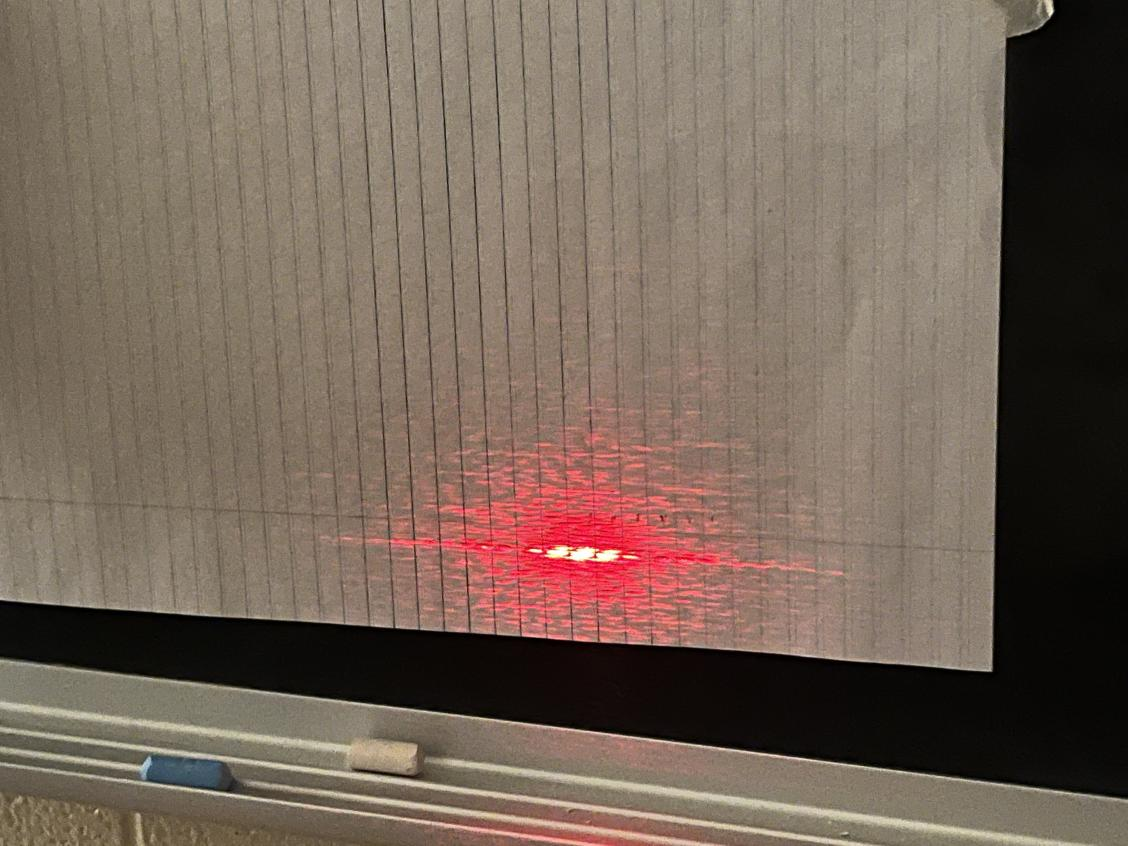
\includegraphics[scale=0.15]{/Users/tristan/Desktop/LaTeX/Physics Light Waves/Young's Double Slit Lab//images/laser_split.png}\end{document}